\documentclass[14pt,russian]{scrartcl}
\let\counterwithout\relax
\let\counterwithin\relax
\usepackage{lmodern}
\usepackage{float}
\usepackage{xcolor}
\usepackage{extsizes}
\usepackage{subfig}
\usepackage[export]{adjustbox}
\usepackage{tocvsec2} % возможность менять учитываемую глубину разделов в оглавлении
\usepackage[subfigure]{tocloft}

\usepackage{fancyvrb}
\usepackage{ulem,bm,mathrsfs,ifsym} %зачеркивания, особо жирный стиль и RSFS начертание
\usepackage{sectsty} % переопределение стилей подразделов
%%%%%%%%%%%%%%%%%%%%%%%

%%% Поля и разметка страницы %%%
\usepackage{pdflscape}                              % Для включения альбомных страниц
\usepackage{geometry}                               % Для последующего задания полей
\geometry{a4paper,tmargin=2cm,bmargin=2cm,lmargin=3cm,rmargin=1cm} % тоже самое, но лучше

%%% Математические пакеты %%%
\usepackage{amsthm,amsfonts,amsmath,amssymb,amscd}  % Математические дополнения от AMS
\usepackage{mathtools}                              % Добавляет окружение multlined
\usepackage[perpage]{footmisc}

%%%% Установки для размера шрифта 14 pt %%%%
%% Формирование переменных и констант для сравнения (один раз для всех подключаемых файлов)%%
%% должно располагаться до вызова пакета fontspec или polyglossia, потому что они сбивают его работу
%\newlength{\curtextsize}
%\newlength{\bigtextsize}
%\setlength{\bigtextsize}{13pt}
\KOMAoptions{fontsize=14pt}

\makeatletter
\def\showfontsize{\f@size{} point}
\makeatother

%\makeatletter
%\show\f@size                                       % неплохо для отслеживания, но вызывает стопорение процесса, если документ компилируется без команды  -interaction=nonstopmode 
%\setlength{\curtextsize}{\f@size pt}
%\makeatother

%шрифт times
\usepackage{tempora}

   %%% Решение проблемы копирования текста в буфер кракозябрами
%    \input glyphtounicode.tex
%    \input glyphtounicode-cmr.tex %from pdfx package
%    \pdfgentounicode=1
    \usepackage{cmap}                               % Улучшенный поиск русских слов в полученном pdf-файле
    \usepackage[T2A]{fontenc}                       % Поддержка русских букв
    \usepackage[utf8]{inputenc}                     % Кодировка utf8
    \usepackage[english, main=russian]{babel}            % Языки: русский, английский
%   \IfFileExists{pscyr.sty}{\usepackage{pscyr}}{}  % Красивые русские шрифты
%\renewcommand{\rmdefault}{ftm}
%%% Оформление абзацев %%%
\usepackage{indentfirst}                            % Красная строка
%\usepackage{eskdpz}

%%% Таблицы %%%
\usepackage{longtable}                              % Длинные таблицы
\usepackage{multirow,makecell,array}                % Улучшенное форматирование таблиц
\usepackage{booktabs}                               % Возможность оформления таблиц в классическом книжном стиле (при правильном использовании не противоречит ГОСТ)

%%% Общее форматирование
\usepackage{soulutf8}                               % Поддержка переносоустойчивых подчёркиваний и зачёркиваний
\usepackage{icomma}                                 % Запятая в десятичных дробях



%%% Изображения %%%
\usepackage{graphicx}                               % Подключаем пакет работы с графикой
\usepackage{wrapfig}

%%% Списки %%%
\usepackage{enumitem}

%%% Подписи %%%
\usepackage{caption}                                % Для управления подписями (рисунков и таблиц) % Может управлять номерами рисунков и таблиц с caption %Иногда может управлять заголовками в списках рисунков и таблиц
%% Использование:
%\begin{table}[h!]\ContinuedFloat - чтобы не переключать счетчик
%\captionsetup{labelformat=continued}% должен стоять до самого caption
%\caption{}
% либо ручками \caption*{Продолжение таблицы~\ref{...}.} :)

%%% Интервалы %%%

%%% Счётчики %%%
\usepackage[figure,table,section]{totalcount}               % Счётчик рисунков и таблиц
\DeclareTotalCounter{lstlisting}
\usepackage{totcount}                               % Пакет создания счётчиков на основе последнего номера подсчитываемого элемента (может требовать дважды компилировать документ)
\usepackage{totpages}                               % Счётчик страниц, совместимый с hyperref (ссылается на номер последней страницы). Желательно ставить последним пакетом в преамбуле

%%% Продвинутое управление групповыми ссылками (пока только формулами) %%%
%% Кодировки и шрифты %%%

%   \newfontfamily{\cyrillicfont}{Times New Roman}
%   \newfontfamily{\cyrillicfonttt}{CMU Typewriter Text}
	%\setmainfont{Times New Roman}
	%\newfontfamily\cyrillicfont{Times New Roman}
	%\setsansfont{Times New Roman}                    %% задаёт шрифт без засечек
%	\setmonofont{Liberation Mono}               %% задаёт моноширинный шрифт
 %   \IfFileExists{pscyr.sty}{\renewcommand{\rmdefault}{ftm}}{}
%%% Интервалы %%%
%linespread-реализация ближе к реализации полуторного интервала в ворде.
%setspace реализация заточена под шрифты 10, 11, 12pt, под остальные кегли хуже, но всё же ближе к типографской классике. 
\linespread{1.3}                    % Полуторный интервал (ГОСТ Р 7.0.11-2011, 5.3.6)
%\renewcommand{\@biblabel}[1]{#1}

%%% Гиперссылки %%%
\usepackage{hyperref}

%%% Выравнивание и переносы %%%
\sloppy                             % Избавляемся от переполнений
\clubpenalty=10000                  % Запрещаем разрыв страницы после первой строки абзаца
\widowpenalty=10000                 % Запрещаем разрыв страницы после последней строки абзаца

\makeatletter % малые заглавные, small caps shape
\let\@@scshape=\scshape
\renewcommand{\scshape}{%
  \ifnum\strcmp{\f@series}{bx}=\z@
    \usefont{T1}{cmr}{bx}{sc}%
  \else
    \ifnum\strcmp{\f@shape}{it}=\z@
      \fontshape{scsl}\selectfont
    \else
      \@@scshape
    \fi
  \fi}
\makeatother

%%% Подписи %%%
%\captionsetup{%
%singlelinecheck=off,                % Многострочные подписи, например у таблиц
%skip=2pt,                           % Вертикальная отбивка между подписью и содержимым рисунка или таблицы определяется ключом
%justification=centering,            % Центрирование подписей, заданных командой \caption
%}
%%%        Подключение пакетов                 %%%
\usepackage{ifthen}                 % добавляет ifthenelse
%%% Инициализирование переменных, не трогать!  %%%
\newcounter{intvl}
\newcounter{otstup}
\newcounter{contnumeq}
\newcounter{contnumfig}
\newcounter{contnumtab}
\newcounter{pgnum}
\newcounter{bibliosel}
\newcounter{chapstyle}
\newcounter{headingdelim}
\newcounter{headingalign}
\newcounter{headingsize}
\newcounter{tabcap}
\newcounter{tablaba}
\newcounter{tabtita}
%%%%%%%%%%%%%%%%%%%%%%%%%%%%%%%%%%%%%%%%%%%%%%%%%%

%%% Область упрощённого управления оформлением %%%

%% Интервал между заголовками и между заголовком и текстом
% Заголовки отделяют от текста сверху и снизу тремя интервалами (ГОСТ Р 7.0.11-2011, 5.3.5)
\setcounter{intvl}{3}               % Коэффициент кратности к размеру шрифта

%% Отступы у заголовков в тексте
\setcounter{otstup}{0}              % 0 --- без отступа; 1 --- абзацный отступ

%% Нумерация формул, таблиц и рисунков
\setcounter{contnumeq}{1}           % Нумерация формул: 0 --- пораздельно (во введении подряд, без номера раздела); 1 --- сквозная нумерация по всей диссертации
\setcounter{contnumfig}{1}          % Нумерация рисунков: 0 --- пораздельно (во введении подряд, без номера раздела); 1 --- сквозная нумерация по всей диссертации
\setcounter{contnumtab}{1}          % Нумерация таблиц: 0 --- пораздельно (во введении подряд, без номера раздела); 1 --- сквозная нумерация по всей диссертации

%% Оглавление
\setcounter{pgnum}{0}               % 0 --- номера страниц никак не обозначены; 1 --- Стр. над номерами страниц (дважды компилировать после изменения)

%% Библиография
\setcounter{bibliosel}{1}           % 0 --- встроенная реализация с загрузкой файла через движок bibtex8; 1 --- реализация пакетом biblatex через движок biber

%% Текст и форматирование заголовков
\setcounter{chapstyle}{1}           % 0 --- разделы только под номером; 1 --- разделы с названием "Глава" перед номером
\setcounter{headingdelim}{1}        % 0 --- номер отделен пропуском в 1em или \quad; 1 --- номера разделов и приложений отделены точкой с пробелом, подразделы пропуском без точки; 2 --- номера разделов, подразделов и приложений отделены точкой с пробелом.

%% Выравнивание заголовков в тексте
\setcounter{headingalign}{0}        % 0 --- по центру; 1 --- по левому краю

%% Размеры заголовков в тексте
\setcounter{headingsize}{0}         % 0 --- по ГОСТ, все всегда 14 пт; 1 --- пропорционально изменяющийся размер в зависимости от базового шрифта

%% Подпись таблиц
\setcounter{tabcap}{0}              % 0 --- по ГОСТ, номер таблицы и название разделены тире, выровнены по левому краю, при необходимости на нескольких строках; 1 --- подпись таблицы не по ГОСТ, на двух и более строках, дальнейшие настройки: 
%Выравнивание первой строки, с подписью и номером
\setcounter{tablaba}{2}             % 0 --- по левому краю; 1 --- по центру; 2 --- по правому краю
%Выравнивание строк с самим названием таблицы
\setcounter{tabtita}{1}             % 0 --- по левому краю; 1 --- по центру; 2 --- по правому краю

%%% Рисунки %%%
\DeclareCaptionLabelSeparator*{emdash}{~--- }             % (ГОСТ 2.105, 4.3.1)
\captionsetup[figure]{labelsep=emdash,font=onehalfspacing,position=bottom}

%%% Таблицы %%%
\ifthenelse{\equal{\thetabcap}{0}}{%
    \newcommand{\tabcapalign}{\raggedright}  % по левому краю страницы или аналога parbox
}

\ifthenelse{\equal{\thetablaba}{0} \AND \equal{\thetabcap}{1}}{%
    \newcommand{\tabcapalign}{\raggedright}  % по левому краю страницы или аналога parbox
}

\ifthenelse{\equal{\thetablaba}{1} \AND \equal{\thetabcap}{1}}{%
    \newcommand{\tabcapalign}{\centering}    % по центру страницы или аналога parbox
}

\ifthenelse{\equal{\thetablaba}{2} \AND \equal{\thetabcap}{1}}{%
    \newcommand{\tabcapalign}{\raggedleft}   % по правому краю страницы или аналога parbox
}

\ifthenelse{\equal{\thetabtita}{0} \AND \equal{\thetabcap}{1}}{%
    \newcommand{\tabtitalign}{\raggedright}  % по левому краю страницы или аналога parbox
}

\ifthenelse{\equal{\thetabtita}{1} \AND \equal{\thetabcap}{1}}{%
    \newcommand{\tabtitalign}{\centering}    % по центру страницы или аналога parbox
}

\ifthenelse{\equal{\thetabtita}{2} \AND \equal{\thetabcap}{1}}{%
    \newcommand{\tabtitalign}{\raggedleft}   % по правому краю страницы или аналога parbox
}

\DeclareCaptionFormat{tablenocaption}{\tabcapalign #1\strut}        % Наименование таблицы отсутствует
\ifthenelse{\equal{\thetabcap}{0}}{%
    \DeclareCaptionFormat{tablecaption}{\tabcapalign #1#2#3}
    \captionsetup[table]{labelsep=emdash}                       % тире как разделитель идентификатора с номером от наименования
}{%
    \DeclareCaptionFormat{tablecaption}{\tabcapalign #1#2\par%  % Идентификатор таблицы на отдельной строке
        \tabtitalign{#3}}                                       % Наименование таблицы строкой ниже
    \captionsetup[table]{labelsep=space}                        % пробельный разделитель идентификатора с номером от наименования
}
\captionsetup[table]{format=tablecaption,singlelinecheck=off,font=onehalfspacing,position=top,skip=-5pt}  % многострочные наименования и прочее
\DeclareCaptionLabelFormat{continued}{Продолжение таблицы~#2}
\setlength{\belowcaptionskip}{.2cm}
\setlength{\intextsep}{0ex}

%%% Подписи подрисунков %%%
\renewcommand{\thesubfigure}{\asbuk{subfigure}}           % Буквенные номера подрисунков
\captionsetup[subfigure]{font={normalsize},               % Шрифт подписи названий подрисунков (не отличается от основного)
    labelformat=brace,                                    % Формат обозначения подрисунка
    justification=centering,                              % Выключка подписей (форматирование), один из вариантов            
}
%\DeclareCaptionFont{font12pt}{\fontsize{12pt}{13pt}\selectfont} % объявляем шрифт 12pt для использования в подписях, тут же надо интерлиньяж объявлять, если не наследуется
%\captionsetup[subfigure]{font={font12pt}}                 % Шрифт подписи названий подрисунков (всегда 12pt)

%%% Настройки гиперссылок %%%

\definecolor{linkcolor}{rgb}{0.0,0,0}
\definecolor{citecolor}{rgb}{0,0.0,0}
\definecolor{urlcolor}{rgb}{0,0,0}

\hypersetup{
    linktocpage=true,           % ссылки с номера страницы в оглавлении, списке таблиц и списке рисунков
%    linktoc=all,                % both the section and page part are links
%    pdfpagelabels=false,        % set PDF page labels (true|false)
    plainpages=true,           % Forces page anchors to be named by the Arabic form  of the page number, rather than the formatted form
    colorlinks,                 % ссылки отображаются раскрашенным текстом, а не раскрашенным прямоугольником, вокруг текста
    linkcolor={linkcolor},      % цвет ссылок типа ref, eqref и подобных
    citecolor={citecolor},      % цвет ссылок-цитат
    urlcolor={urlcolor},        % цвет гиперссылок
    pdflang={ru},
}
\urlstyle{same}
%%% Шаблон %%%
%\DeclareRobustCommand{\todo}{\textcolor{red}}       % решаем проблему превращения названия цвета в результате \MakeUppercase, http://tex.stackexchange.com/a/187930/79756 , \DeclareRobustCommand protects \todo from expanding inside \MakeUppercase
\setlength{\parindent}{2.5em}                       % Абзацный отступ. Должен быть одинаковым по всему тексту и равен пяти знакам (ГОСТ Р 7.0.11-2011, 5.3.7).

%%% Списки %%%
% Используем дефис для ненумерованных списков (ГОСТ 2.105-95, 4.1.7)
%\renewcommand{\labelitemi}{\normalfont\bfseries~{---}} 
\renewcommand{\labelitemi}{\bfseries~{---}} 
\setlist{nosep,%                                    % Единый стиль для всех списков (пакет enumitem), без дополнительных интервалов.
    labelindent=\parindent,leftmargin=*%            % Каждый пункт, подпункт и перечисление записывают с абзацного отступа (ГОСТ 2.105-95, 4.1.8)
}
%%%%%%%%%%%%%%%%%%%%%%
%\usepackage{xltxtra} % load xunicode

\usepackage{ragged2e}
\usepackage[explicit]{titlesec}
\usepackage{placeins}
\usepackage{xparse}

\usepackage{listingsutf8}
\usepackage{url} %пакеты расширений
\usepackage{algorithm, algorithmicx}
\usepackage[noend]{algpseudocode}
\usepackage{blkarray}
\usepackage{chngcntr}
\usepackage{tabularx}
\newcommand*\template[1]{\text{<}#1\text{>}}

  
\titleformat{name=\section,numberless}[block]{\normalfont\Large\centering}{}{0em}{#1}
\titleformat{\section}[block]{\normalfont\Large\bfseries\raggedright}{}{0em}{\thesection\hspace{0.25em}#1}
\titleformat{\subsection}[block]{\normalfont\Large\bfseries\raggedright}{}{0em}{\thesubsection\hspace{0.25em}#1}
\titleformat{\subsubsection}[block]{\normalfont\large\bfseries\raggedright}{}{0em}{\thesubsubsection\hspace{0.25em}#1}

\let\Algorithm\algorithm
\renewcommand\algorithm[1][]{\Algorithm[#1]\setstretch{1.5}}

\usepackage{relsize}
\usepackage{pifont}
\usepackage{calc}
\usepackage{suffix}
\usepackage{csquotes}
\DeclareQuoteStyle{russian}
    {\guillemotleft}{\guillemotright}[0.025em]
    {\quotedblbase}{\textquotedblleft}
\ExecuteQuoteOptions{style=russian}
\newcommand{\enq}[1]{\enquote{#1}}  
\newcommand{\eng}[1]{\begin{english}#1\end{english}}
% Подчиненные счетчики в окружениях http://old.kpfu.ru/journals/izv_vuz/arch/sample1251.tex
\newcounter{cTheorem} 
\newcounter{cDefinition}
\newcounter{cConsequent}
\newcounter{cExample}
\newcounter{cLemma}
\newcounter{cConjecture}
\newtheorem{Theorem}{Теорема}[cTheorem]
\newtheorem{Definition}{Определение}[cDefinition]
\newtheorem{Consequent}{Следствие}[cConsequent]
\newtheorem{Example}{Пример}[cExample]
\newtheorem{Lemma}{Лемма}[cLemma]
\newtheorem{Conjecture}{Гипотеза}[cConjecture]

\renewcommand{\theTheorem}{\arabic{Theorem}}
\renewcommand{\theDefinition}{\arabic{Definition}}
\renewcommand{\theConsequent}{\arabic{Consequent}}
\renewcommand{\theExample}{\arabic{Example}}
\renewcommand{\theLemma}{\arabic{Lemma}}
\renewcommand{\theConjecture}{\arabic{Conjecture}}
%\makeatletter
\NewDocumentCommand{\Newline}{}{\text{\\}}
\newcommand{\sequence}[2]{\ensuremath \left(#1,\ \dots,\ #2\right)}

\definecolor{mygreen}{rgb}{0,0.6,0}
\definecolor{mygray}{rgb}{0.5,0.5,0.5}
\definecolor{mymauve}{rgb}{0.58,0,0.82}
\renewcommand{\listalgorithmname}{Список алгоритмов}
\floatname{algorithm}{Листинг}
\renewcommand{\lstlistingname}{Листинг}
\renewcommand{\thealgorithm}{\arabic{algorithm}}

\newcommand{\refAlgo}[1]{(листинг \ref{#1})}
\newcommand{\refImage}[1]{(рисунок \ref{#1})}

\renewcommand{\theenumi}{\arabic{enumi}.}% Меняем везде перечисления на цифра.цифра	
\renewcommand{\labelenumi}{\arabic{enumi}.}% Меняем везде перечисления на цифра.цифра
\renewcommand{\theenumii}{\arabic{enumii}}% Меняем везде перечисления на цифра.цифра
\renewcommand{\labelenumii}{(\arabic{enumii})}% Меняем везде перечисления на цифра.цифра
\renewcommand{\theenumiii}{\roman{enumiii}}% Меняем везде перечисления на цифра.цифра
\renewcommand{\labelenumiii}{(\roman{enumiii})}% Меняем везде перечисления на цифра.цифра
%\newfontfamily\AnkaCoder[Path=src/fonts/]{AnkaCoder-r.ttf}
\renewcommand{\labelitemi}{---}
\renewcommand{\labelitemii}{---}

%\usepackage{courier}

\graphicspath{ {./img/} }

\lstdefinelanguage{Refal}{
  alsodigit = {.,<,>},
  morekeywords = [1]{$ENTRY},
  morekeywords = [2]{Go, Put, Get, Open, Close, Arg, Add, Sub, Mul, Div, Symb, Explode, Implode},
  %keyword4
  morekeywords = [3]{<,>},
  %keyword5
  morekeywords = [4]{e.,t.,s.},
  sensitive = true,
  morecomment = [l]{*},
  morecomment = [s]{/*}{*/},
  commentstyle = \color{mygreen},
  morestring = [b]",
  morestring = [b]',
  stringstyle = \color{purple}
}

\makeatletter
\def\p@subsection{}
\def\p@subsubsection{\thesection\,\thesubsection\,}
\makeatother
\newcommand{\prog}[1]{{\ttfamily\small#1}}
\lstset{ %
  backgroundcolor=\color{white},   % choose the background color; you must add \usepackage{color} or \usepackage{xcolor}
  basicstyle=\ttfamily\footnotesize, 
  %basicstyle=\footnotesize\AnkaCoder,        % the size of the fonts that are used for the code
  breakatwhitespace=false,         % sets if automatic breaks shoulbd only happen at whitespace
  breaklines=true,                 % sets automatic line breaking
  captionpos=top,                    % sets the caption-position to bottom
  commentstyle=\color{mygreen},    % comment style
  deletekeywords={...},            % if you want to delete keywords from the given language
  escapeinside={\%*}{*)},          % if you want to add LaTeX within your code
  extendedchars=true,              % lets you use non-ASCII characters; for 8-bits encodings only, does not work with UTF-8
  inputencoding=utf8,
  frame=single,                    % adds a frame around the code
  keepspaces=true,                 % keeps spaces in text, useful for keeping indentation of code (possibly needs columns=flexible)
  keywordstyle=\bf,       % keyword style
  language=Refal,                    % the language of the code
  morekeywords={<,>,$ENTRY,Go,Arg, Open, Close, e., s., t., Get, Put}, 
  							       % if you want to add more keywords to the set
  numbers=left,                    % where to put the line-numbers; possible values are (none, left, right)
  numbersep=5pt,                   % how far the line-numbers are from the code
  xleftmargin=25pt,
  xrightmargin=25pt,
  numberstyle=\small\color{black}, % the style that is used for the line-numbers
  rulecolor=\color{black},         % if not set, the frame-color may be changed on line-breaks within not-black text (e.g. comments (green here))
  showspaces=false,                % show spaces everywhere adding particular underscores; it overrides 'showstringspaces'
  showstringspaces=false,          % underline spaces within strings only
  showtabs=false,                  % show tabs within strings adding particular underscores
  stepnumber=1,                    % the step between two line-numbers. If it's 1, each line will be numbered
  stringstyle=\color{mymauve},     % string literal style
  tabsize=8,                       % sets default tabsize to 8 spaces
  title=\lstname                   % show the filename of files included with \lstinputlisting; also try caption instead of title
}
\newcommand{\anonsection}[1]{\cleardoublepage
\phantomsection
\addcontentsline{toc}{section}{\protect\numberline{}#1}
\section*{#1}\vspace*{2.5ex} % По госту положены 3 пустые строки после заголовка ненумеруемого раздела
}
\newcommand{\sectionbreak}{\clearpage}
\renewcommand{\sectionfont}{\normalsize} % Сбиваем стиль оглавления в стандартный
\renewcommand{\cftsecleader}{\cftdotfill{\cftdotsep}} % Точки в оглавлении напротив разделов

\renewcommand{\cftsecfont}{\normalfont\large} % Переключение на times в содержании
\renewcommand{\cftsubsecfont}{\normalfont\large} % Переключение на times в содержании

\usepackage{caption} 
%\captionsetup[table]{justification=raggedleft} 
%\captionsetup[figure]{justification=centering,labelsep=endash}
\usepackage{amsmath}    % \bar    (матрицы и проч. ...)
\usepackage{amsfonts}   % \mathbb (символ для множества действительных чисел и проч. ...)
\usepackage{mathtools}  % \abs, \norm
    \DeclarePairedDelimiter\abs{\lvert}{\rvert} % операция модуля
    \DeclarePairedDelimiter\norm{\lVert}{\rVert} % операция нормы
\DeclareTextCommandDefault{\textvisiblespace}{%
  \mbox{\kern.06em\vrule \@height.3ex}%
  \vbox{\hrule \@width.3em}%
  \hbox{\vrule \@height.3ex}}    
\newsavebox{\spacebox}
\begin{lrbox}{\spacebox}
\verb*! !
\end{lrbox}
\newcommand{\aspace}{\usebox{\spacebox}}

\title{Lab 02 report}
\author{Gadzhi}

\date{\today}

\begin{document}
\thispagestyle{empty}

\noindent \begin{minipage}{0.15\textwidth}
	
\includegraphics[width=\linewidth]{b_logo}
\end{minipage}
\noindent\begin{minipage}{0.85\textwidth}\centering
	\textbf{Министерство науки и высшего образования Российской Федерации}\\
	\textbf{Федеральное государственное бюджетное образовательное учреждение высшего образования}\\
	\textbf{«Московский государственный технический университет имени Н.Э.~Баумана}\\
	\textbf{(национальный исследовательский университет)»}\\
	\textbf{(МГТУ им. Н.Э.~Баумана)}
\end{minipage}

\noindent\rule{16cm}{3pt}
\newline\newline
\noindent ФАКУЛЬТЕТ $\underline{\text{«Информатика и системы управления»}}$ \newline\newline
\noindent КАФЕДРА $\underline{\text{«Программное обеспечение ЭВМ и информационные технологии»}}$\newline


\begin{center}
	\noindent\begin{minipage}{1.3\textwidth}\centering
	\Large\textbf{   ~~~ Лабораторная работа №4}\newline
	\textbf{по дисциплине "Анализ Алгоритмов"}\newline\newline\newline
	\end{minipage}
\end{center}

\noindent\textbf{Тема} $\underline{\text{Параллельное программирование}}$\newline\newline
\noindent\textbf{Студент} $\underline{\text{Кишов Г. М.}}$\newline\newline
\noindent\textbf{Группа} $\underline{\text{ИУ7-53Б}}$\newline\newline
\noindent\textbf{Преподаватель} $\underline{\text{Волкова Л. Л.}}$\newline

\begin{center}
	\mbox{}
	\vfill
	Москва
\end{center}

\begin{center}
	\the\year ~г.
\end{center}
\clearpage

\renewcommand\contentsname{\hfill{\normalfont{СОДЕРЖАНИЕ}}\hfill}  %Оглавление
\tableofcontents
\newpage

\anonsection{Введение}

Многопоточность - способность центрального процессора (CPU) или одного ядра в многоядерном процессоре одновременно выполнять несколько процессов или потоков, соответствующим образом поддерживаемых операционной системой. Смысл многопоточности - квазимногозадачность на уровне одного исполняемого процесса. Данный подход не стоит путать с многопроцессорностью, так как многопоточность процессов и потоков совместно использует ресурсы одного или нескольких ядер: кэш-памяти CPU, вычислительных блоков.

В случаях, когда многопроцессорные системы включают в себя несколько полных блоков обработки, многопоточность направлена на максимизацию использования ресурсов одного ядра.

Так как эти два метода являются взаимодополняющими, то их иногда объединяют в системах с несколькими многопоточными ЦП и в ЦП с нескольким многопоточными ядрами. 

\textbf{Цель лабораторной работы:} изучение параллельных вычислений на примере нахождения среднего геометрического строк матрицы.

\textbf{Для достижения поставленной цели необходимо выполнить следующие задачи:}

\begin{itemize}
    \item Исследовать основы параллельных вычислений;
    \item Привести схемы реализации последовательного и параллельного подсчета среднего геометрического строк матрицы;
    \item Определить средства программной реализации;
    \item Протестировать разработанное программное обеспечение;
    \item Провести сравнительный анализ временных характеристик алгоритмов;
    \item На основании проделанной работы сделать выводы.
\end{itemize}

\section{Аналитический раздел}

В данном разделе будет рассмотрен алгоритм нахождения среднего геометрического строк матрицы и его параллельная реализация.

\subsection{Некоторые теоретические сведения}

Средним геометрическим [1] ряда положительных чисел называется такое число, которым можно заменить каждое из данных чисел так, чтобы их произведение не изменилось. Другими словами, среднее геометрическое \textit{n} чисел равно корню \textit{n-ой} степени из их произведения.

Формула вычисления среднего геометрического \textit{n} чисел:

\begin{equation}
    \displaystyle
    G(x_{1}, x_{2} \cdots x_{n}) = \displaystyle\sqrt[1/n]{\prod_{i = 1}^{n} x_{i}}  
\end{equation}

\subsection{Алгоритм нахождения среднего геометрического строк матрицы}

Пусть дана прямоугольная матрица

\begin{equation}
    A_{nm} =
      \begin{pmatrix}
        a_{11} & a_{12} & \cdots & a_{1m} \\
        a_{21} & a_{22} & \cdots & a_{2m} \\
        \vdots & \vdots & \ddots & \vdots \\
        a_{n1} & a_{n2} & \cdots & a_{nm}
      \end{pmatrix},
\end{equation}

\vspace{5mm}

Тогда средним геометрическим строк матрицы \textit{A} будет называться массив \textit{B}

\begin{equation}
    B{n} =
    \begin{pmatrix}
      b_{1} & b_{2} & \cdots & b_{n} \\
    \end{pmatrix},
\end{equation}

где

\begin{equation}
    \displaystyle
    B[i] = \displaystyle\sqrt[1/m]{\prod_{j = 1}^{m} a_{ij}}, \quad (i = \overline{1, n})  
\end{equation}

Среднее геометрическое \textit{i-ой} строки матрицы \textit{A}.

\subsection{Параллельный алгоритм нахождения среднего геометрического строк матрицы}

Поскольку каждый элемент массива \textit{B} вычисляется независимо от других и матрица \textit{A} не изменяется в процессе, то для распараллеливания алгоритма нахождения среднего геометрического строк матрицы достаточно равным образом распределить строки матрицы \textit{А} между потоками.

\subsection{Вывод}

В данном разделе были рассмотрены последовательный и параллельный алгоритмы нахождения среднего геометрического строк матрицы. 

В качестве входных данных в программу будут подаваться целочисленная матрица, ее размер (количество строк и столбцов матрицы). На выходе программа будет выдавать массив, который будет содержать средние геометрические каждой строки исходной матрицы. Ограничением для работы программного продукта будет являться то, что размеры матриц должны быть целыми положительными числами, а сами матрицы состоять только из положительных целочисленных значений. 

Реализуемое программное обеспечение будет работать в пользовательском и экспериментальном режимах. В пользовательском режиме можно будет ввести матрицу и программа выведет среднее геометрическое строк данной матрицы, в экспериментальном режиме будет проводиться сравнение временных характеристик последовательного и параллельного алгоритма нахождения среднего геометрического строк матрицы при разном количестве потоков.

\section{Конструкторский раздел}

В данном разделе будут представлены схемы алгоритмов, описаны используемые типы данных, структура программного обеспечения (далее - ПО) и классы эквивалентности.

\subsection{Схемы алгоритмов}

На рисунках \ref{fig:classic}-\ref{fig:parallel_additional} приведены схемы реализации алгоритмов последовательного и параллельного нахождения среднего геометрического строк матрицы.

\begin{figure}[h]
	\centering
	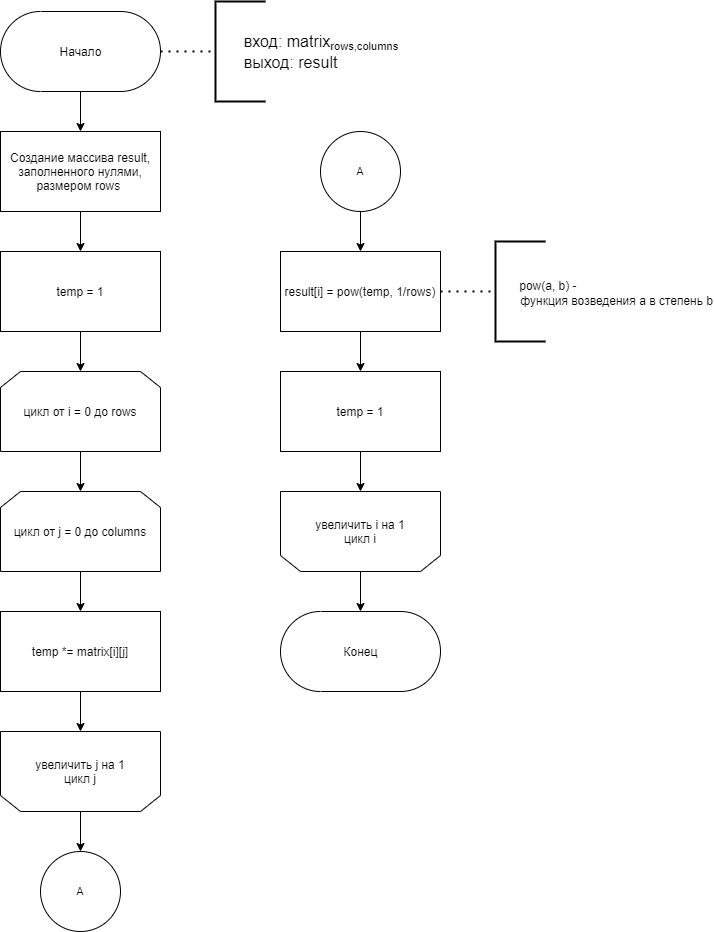
\includegraphics[scale=0.6]{classic.png}
	\caption{Схема последовательного алгоритма нахождения среднего геометрического строк матрицы}
	\label{fig:classic}
\end{figure}

\begin{figure}[h]
	\centering
	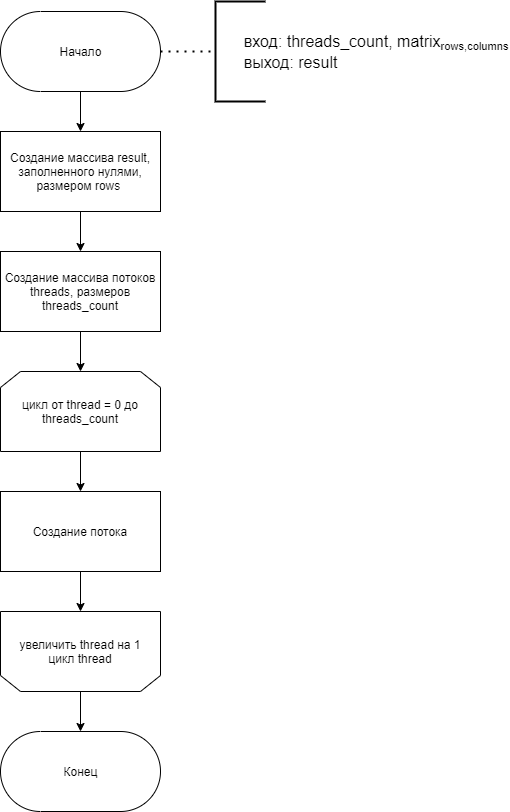
\includegraphics[scale=0.7]{parallel.png}
	\caption{Схема параллельного алгоритма нахождения среднего геометрического строк матрицы}
	\label{fig:parallel}
\end{figure}

\begin{figure}[h]
	\centering
	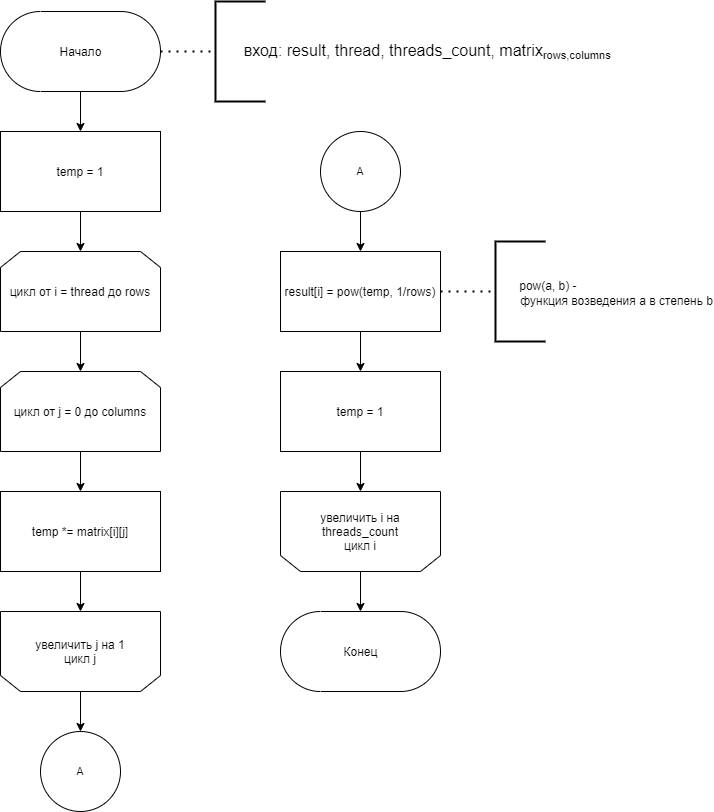
\includegraphics[scale=0.6]{parallel_additional.png}
	\caption{Схема создания одного потока}
	\label{fig:parallel_additional}
\end{figure}

\clearpage

\subsection{Описание используемых типов данных}

При реализации алгоритмов будут использованы следующие структуры данных:
		
\begin{enumerate}
    \item количество строк матрицы - целое число типа \text{int};
    \item количество столбцов матрицы - целок число типа \text{int};
    \item матрица - двумерный массив типа \text{int};
    \item результирующий массив - одномерный массив типа \text{int};
    \item массив потоков - одномерны массив типа \text{thread}.
\end{enumerate}

\subsection{Структура ПО}

ПО будет состоять из двух модулей:
		
\begin{enumerate}
	\item \textit{main.cpp} - модуль, содержащий весь служебный код;
	\item \textit{algos.cpp} - модуль, содержащий код алгоритмов нахождения среднего геометрического строк матрицы.
\end{enumerate}

\subsection{Способы тестирования и классы эквивалентности}

При тестировании алгоритмов была выбрана методика тестирования черным ящиком. Были выделены следующие классы эквивалентности:

\begin{enumerate}
	\item Матрица заполненная случайными положительными числами;
	\item Матрица, заполненная построчно равными элементами;
	\item Матрица, содержащая один элемент;
	\item Пустая матрица.
\end{enumerate}
\subsection{Вывод} 

В данном разделе были построены схемы алгоритмов нахождения среднего геометрического строк матрицы, описаны используемые типы данных, структура ПО, способы тестирования и классы эквивалентности.

\section{Технологический раздел}

В данном разделе приведены средства реализации и листинги реализаций алгоритмов и тестирование.

\subsection{Средства реализации}

Для реализации программ был выбран язык программирования C++ [2]. Данный язык был выбран поскольку я ознакомился с ним из курса Объектно-ориентированного программирования, а также он предоставляет инструменты для замера процессорного времени и удобной работы с потоками. 

Для работы с потоками использовалась библиотека thread [3]. 

\subsection{Листинги}

\begin{center}
\captionsetup{justification=raggedright,singlelinecheck=off}
\begin{lstlisting}[caption=Функция последовательного нахождения среднего геометрического строк матрицы, label=list:canon, language={}]
double *find_geometric_mean(matrix_s matrix)
{
    double *result = (double*) calloc(matrix.rows, sizeof(double));

    long long int temp = 1;

    for (int i = 0; i < matrix.rows; i++)
    {
        for (int j = 0; j < matrix.columns; j++)
        {
            temp *= matrix.matrix[i][j];
        }

        result[i] = pow(temp, 1.0/matrix.rows);
        temp = 1;
    }

    return result;
}
\end{lstlisting}
\end{center}

\begin{center}
\captionsetup{justification=raggedright,singlelinecheck=off}
\begin{lstlisting}[caption=Функция создания потоков, label=list:vinograd, language={}]
double* parallel_geometric_mean(matrix_s matrix, int threads_count)
{
    double *result = (double*) calloc(matrix.rows, sizeof(double));

    vector<thread> threads(threads_count);

    for (int thread = 0; thread < threads_count; thread++)
    {
        threads[thread] = std::thread(parallel_additional, ref(result), matrix, thread, threads_count);
    }

    for (int i = 0; i < threads_count; i++)
    {
        threads[i].join();
    }

    return result;
}
\end{lstlisting}
\end{center}

\begin{center}
\captionsetup{justification=raggedright,singlelinecheck=off}
\begin{lstlisting}[caption=Функция параллельного нахождения среднего геометрического строк матрицы, label=list:vinograd, language={}]
void parallel_additional(double *result, matrix_s matrix, int thread, int threads_count)
{
    long long int temp = 1;

    for (int i = thread; i < matrix.rows; i += threads_count)
    {
        for (int j = 0; j < matrix.columns; j++)
        {
            temp *= matrix.matrix[i][j];
        }

        result[i] = pow(temp, 1.0/matrix.rows);
        temp = 1;
    }
}
\end{lstlisting}
\end{center}

\subsection{Тестирование функций}

В таблице \ref{tab:tests} приведены модульные тесты для функций умножения матриц выше перечисленными методами. Все тесты были пройдены успешно. \\

\begin{table}[ht]
    \caption{\centering Тестирование функций нахождения среднего геометрического строк матрицы}
    \centering
    \begin{tabular}{|c|c|}
    \hline
    Матрица & Ожидаемый результат \\ \hline
    $\begin{pmatrix}
        2 & 8 & 5 \\
        1 & 10 & 5 \\
        9 & 9 & 3
    \end{pmatrix}$
    &$\begin{pmatrix}
        4.30887 & 3.68403 & 6.24025 \\
    \end{pmatrix}$\\
    \hline
    $\begin{pmatrix}
        1 & 1 \\
        4 & 4
    \end{pmatrix}$
    &$\begin{pmatrix}
        1 & 4 \\
    \end{pmatrix}$\\
    \hline
    $\begin{pmatrix}
        8
    \end{pmatrix}$
    &$\begin{pmatrix}
        8
    \end{pmatrix}$\\
    \hline
    $\begin{pmatrix}
        \\
    \end{pmatrix}$
    &Пусто\\
    \hline
    \end{tabular}
    \label{tab:tests}
    \end{table}

\subsection{Вывод}

Были разработаны и протестированы последовательная и параллельная реализации алгоритма нахождения среднего геометрического строк матрицы. Также было проведено тестирование и описаные средства реализации.

\section{Исследовательский раздел}

В данном разделе будут представлены технические характеристики машины, замер времени выполнения алгоритмов и пример работы программы.

\subsection{Технические характеристики}

Технические характеристики устройства, на котором выполнялось тестирование представлены далее.

\begin{itemize}
    \item Операционная система: Windows 10;
    \item Память: 16 GB 3133 MHz DDR4;
    \item Процессор: Intel® Core™ i7-10700K CPU @ 3.80GHz [4];
    \item 8 физических и 16 логических ядер.
\end{itemize}

Тестирование проводилось на компьютере, включенном в сеть электропитания.
Во время Тестирования компьютер был нагружен только встроенными приложениями окружения рабочего стола.

\subsection{Пример работы программы}

Демонстрация работы программы приведена на рисунке 6.
\vspace{5mm}

\begin{figure}[h]
	\begin{center}
	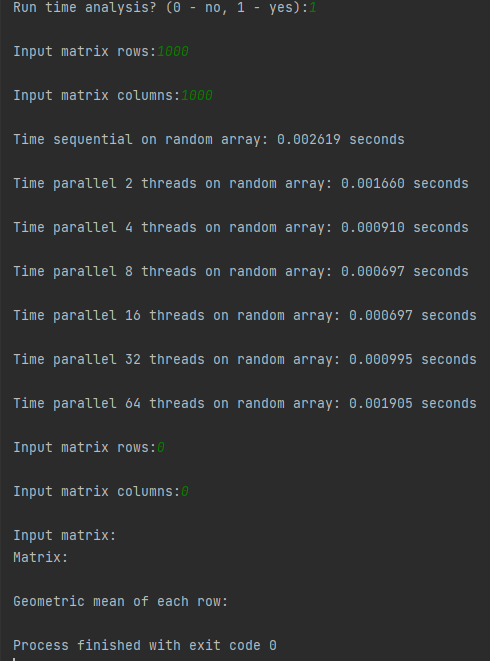
\includegraphics[scale=1]{example.png}
	 \caption{Пример работы программы.}
	\end{center}
\end{figure}

\clearpage

\subsection{Время выполнения алгоритмов}

Был проведен замер времени работы каждого из алгоритмов с помощью библиотеки chrono [5]. Эта библиотека замеряет процессорное время выполнения функции. При выполнении алгоритма проводилось 20 замеров и полученное время усреднялось. В таблице \ref{tab:time_threads} содержаться временные характеристики параллельной реализации алгоритма при размере матрицы 10000х10000 и при разном количестве потоков. В таблице \ref{tab:time_comp} приводится сравнение времени работы последовательной и параллельной реализации алгоритма при 16 потоках на разных размерах матриц.

На рисунке \ref{img:plot_best} демонстрируется сравнение временных характеристик параллельной реализации алгоритма при размере матрицы 10000х10000 и при разном количестве потоков. На рисунке \ref{img:plot_worst} демонстрируется сравнение времени работы последовательной и параллельной реализации алгоритма при 16 потоках на разных размерах матриц. \\

\begin{table}[ht]
    \caption{\centering Время выполнения параллельной реализации алгоритма (в секундах) при размере матрицы 10000х10000}
    \centering
    \begin{tabular}{|c|c|}
    \hline
    Количество потоков & Параллельная реализация алгоритма \\ \hline
    1     & 0.265104      \\ \hline
    2     & 0.133861      \\ \hline
    4     & 0.069908      \\ \hline
    8     & 0.053910      \\ \hline
    16    & 0.046719      \\ \hline
    32    & 0.047453      \\ \hline
    64    & 0.048590      \\ \hline
    \end{tabular}
    \label{tab:time_threads}
\end{table}

\begin{table}[p]
    \caption{\centering Время выполнения реализаций алгоритмов (в секундах) при 16 потоках}
    \centering
    \begin{tabular}{|c|c|c|}
    \hline
    Размер матрицы & Последовательный алгоритм & Параллельный алгоритм\\ \hline
    1000х1000      & 0.002669 & 0.000737 \\ \hline
    5000х5000      & 0.066974 & 0.009691 \\ \hline
    10000х10000    & 0.264854 & 0.046719 \\ \hline
    15000х15000    & 0.616687 & 0.076846 \\ \hline
    20000х20000    & 1.075421 & 0.137248 \\ \hline
    \end{tabular}
    \label{tab:time_comp}
\end{table}

\clearpage

\begin{figure}
    \centering
    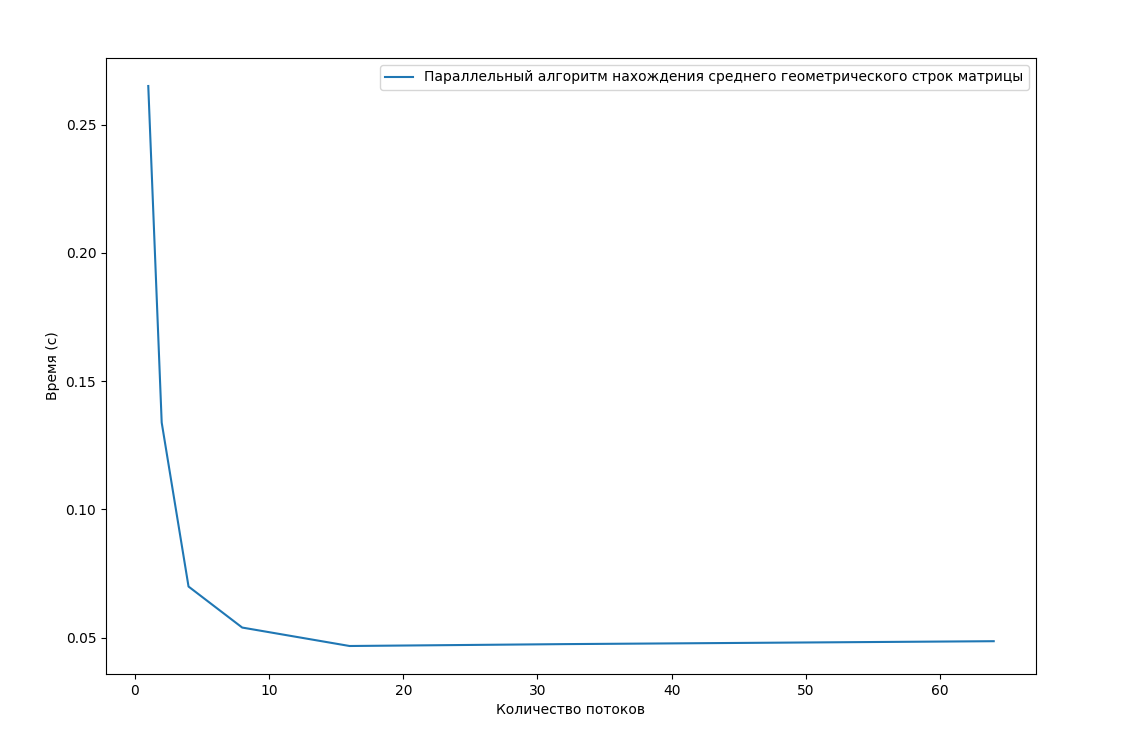
\includegraphics[scale=0.5]{plot_best.png}
    \caption{Зависимость времени выполнения параллельной реализации алгоритма от количества потоков при размере матрицы 10000х10000}
    \label{img:plot_best}
\end{figure}

\begin{figure}
    \centering
    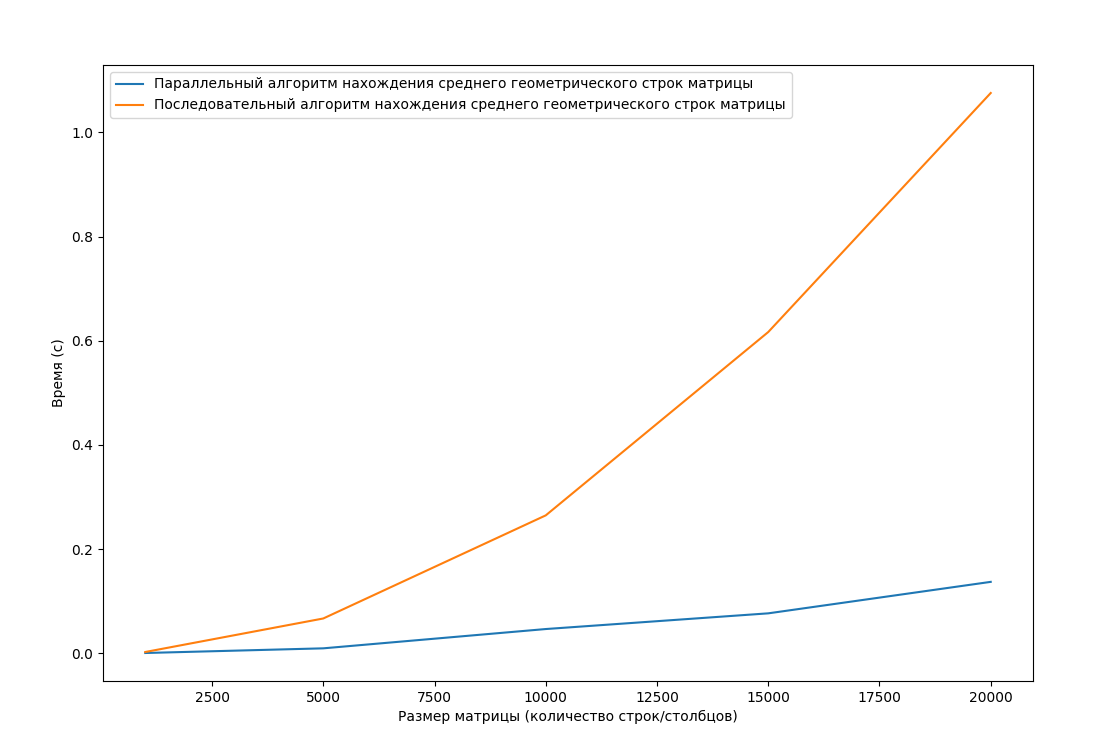
\includegraphics[scale=0.5]{plot_worst.png}
    \caption{Зависимость времени выполнения реализаций алгоритмов от размера матрицы при 16 потоках}
    \label{img:plot_worst}
\end{figure}

\clearpage

\subsection{Вывод}

В данном разделе были описаны технические характеристики машины, приведен пример работы программы и проанализированы временные характеристики алгоритмов нахождения среднего геометрического строк матрицы.

По результатам экспериментов, можно заметить, что лучшее время наблюдается при 16 потоках (быстрее последовательной реализации в 5.7 раз), поскольку мой процессор обладает 16-ю логичскими ядрами, а следовательно максимально одновременно может быть запущено 16 потоков. При количестве потоков больше 16 замечается остановка прогрессии по уменьшению времени работы алгоритма, так как происходит создание очереди самих потоков (если задать 32 потока, то процессор сможет одновременно выполнять только 16 их них, остальные будут ждать своей очереди).
Также стоит заметить, что даже при двух потоках время работы алгоритма уменьшилось примерно в 2 раза, а при четырех потоках, примерно в 4 раза.

\anonsection{Заключение}

В результате выполнения лабораторной работы было экспериментально подтверждено различие временных характеристик последовательной и параллельной реализации алгоритма нахождения среднего геометрического строк матрицы.

В результате исследования временных характеристик можно сделать вывод, что пиковый прирост по времени приходится на 16 потоков (быстрее последовательной реализации в 5.7 раз), посколько процессор, на которым выполнялись замеры имеет 16 логических ядер.

В ходе выполнения работы была достигнута цель и выполнены все поставленные задачи:

\begin{itemize}
    \item Были исследованы основы параллельных вычислений;
    \item Были приведены схемы требуемых алгоритмов;
    \item Были определены средства программной реализации;
    \item Было протестированно разработанное ПО;
    \item Был проведен сравнительный анализ временных характеристик алгоритмов;
    \item На основанни проделанной работы были сделаны соответствующие выводы.
\end{itemize}

\anonsection{Список литературы}

\begin{enumerate}
    \item Среднее геометрическое ряда чисел [Электронный ресурс] Режим доступа: \url{https://umath.ru/calc/srednee-arifmeticheskoe-i-srednee-geometricheskoe-chisel-onlajn/} (дата обращения: 06.11.2021).
    \item Бьёрн Страуструп. Язык программирования C++. Специальное издание = The C++ programming language. Special edition. — Бином-Пресс, 2007. — 1104 с. — ISBN 5-7989-0223-4.
    \item Библиотека для работы с потоками thread [Электронный ресурс] Режис доступа: \url{https://en.cppreference.com/w/cpp/thread} (дата обращения: 06.11.2021).
    \item Процессор Intel® Core™ i7-10700K [Электронный ресурс] Режим доступа: \url{https://www.intel.ru/content/www/ru/ru/products/sku/199335/intel-core-i710700k-processor-16m-cache-up-to-5-10-ghz/specifications.html} (дата обращения: 06.11.2021).
    \item Библиотека Chrono [Электронный ресурс] Режим доступа: \url{https://en.cppreference.com/w/cpp/chrono} (дата обращения: 06.11.2021).
\end{enumerate}

\end{document}